\documentclass[aspectratio=169,10pt]{beamer}
\usetheme{default}
\usecolortheme{seahorse}
\setbeamertemplate{navigation symbols}{}
\setbeamertemplate{footline}[frame number]
\usepackage[T1]{fontenc}
\usepackage{lmodern,booktabs,graphicx}
\graphicspath{{../}}

\title{Design Pattern Analysis in a Node.js/Express Ride-Sharing Application}
\subtitle{23CSE455 Case Study -- Team A6}
\author{Dilip Kumar Reddy \and Sai Sameer \and M Kumar \and K Harish \and S Leela Shankar}
\date{2026-10-11}

\begin{document}
\frame{\titlepage}

\begin{frame}{Application: Sarathi backend}
\begin{columns}[T]
\column{0.42\textwidth}
\small
\begin{itemize}
\item github.com/AkhilMM2000/sarathi-backend, commit \texttt{c8766f4}
\item TypeScript, Express 4, Mongoose, tsyringe DI, Socket.IO + Redis, Stripe, Google Distance Matrix
\item Areas studied: rider, driver, trip, payment, matching, location, notification
\item Matching: 30\,km \texttt{\$geoNear} $\rightarrow$ 20\,km road distance $\rightarrow$ broadcast; first driver to accept wins
\item No upstream license; no tests -- we wrote 14 characterization tests
\end{itemize}
\column{0.58\textwidth}
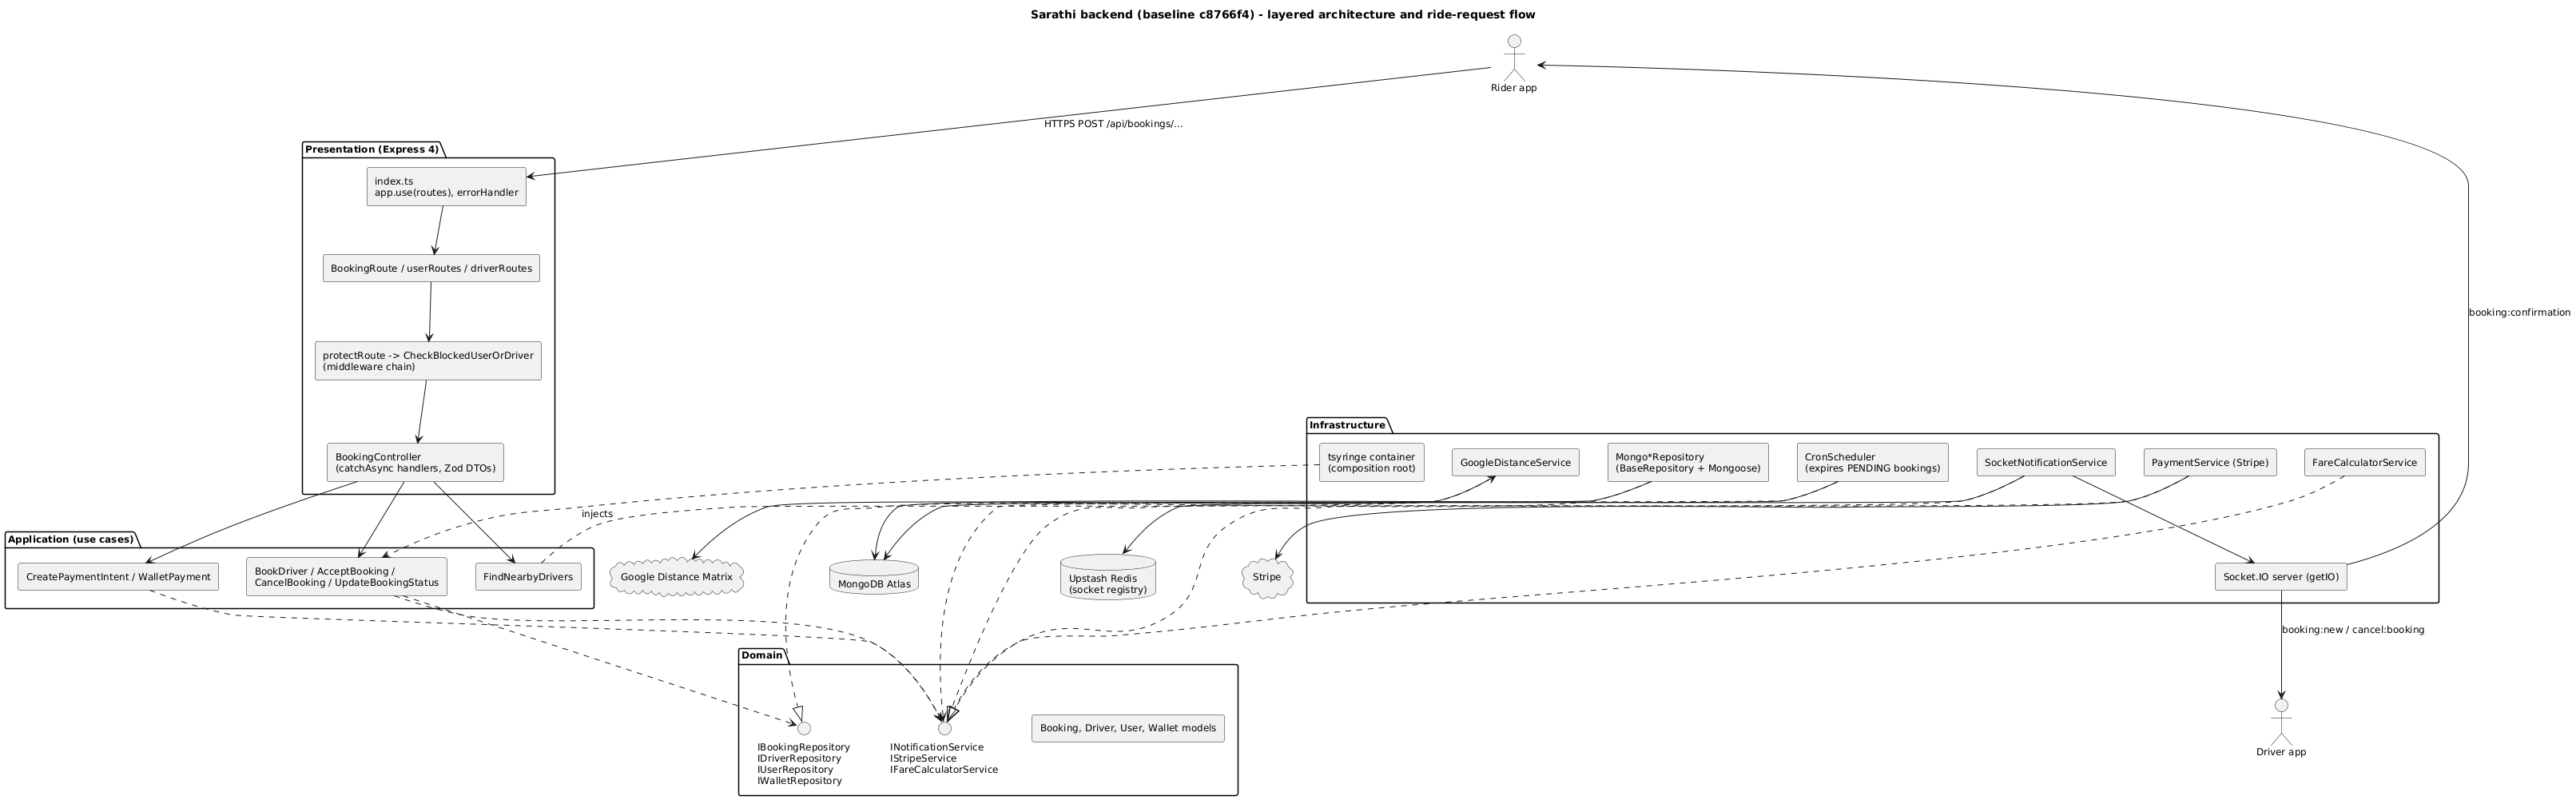
\includegraphics[width=\linewidth]{Part1/diagrams/architecture.png}
\end{columns}
\end{frame}

\begin{frame}{Part 1 -- patterns actually used (baseline)}
\small
\begin{tabular}{@{}lrl@{}}\toprule Pattern & Inst. & Example instance\\\midrule
Layered Architecture & 1 & Ride Booking Request Flow\\
Dependency Injection & 1 & tsyringe composition root\\
Singleton & 1 & Shared Socket.IO server (\texttt{getIO})\\
Repository & 5 & Trip, Driver (geo query), Rider, Wallet, Review\\
Data Mapper & 1 & Driver review mapping\\
Adapter & 3 & Socket.IO notification, Stripe payment, Stripe Connect\\
Gateway & 1 & Google Distance Matrix\\
Observer & 1 & Ride event notification (Redis socket registry)\\
Chain of Responsibility & 1 & \texttt{protectRoute} $\rightarrow$ \texttt{checkBlocked} $\rightarrow$ controller\\
Decorator & 1 & \texttt{catchAsync} error forwarding\\\bottomrule
\end{tabular}

\medskip
\textbf{10 types, 16 instances.} Rejected: Strategy, State, Command, Template Method, Factory Method, Facade. Uncertain: unused Google Maps and Twilio adapters.
\end{frame}

\begin{frame}{What was missing -- and the defects it caused}
\begin{itemize}
\item Fare by ride type: \texttt{if/else} in \texttt{FareCalculatorService}; Rs 10/km duplicated in \texttt{UpdateBookingStatus}
\item Trip and driver status: plain strings + scattered checks
\begin{itemize}
\item a \textbf{COMPLETED trip could be cancelled} (baseline test passes)
\item an admin could move a \textbf{rejected driver straight to approved}
\end{itemize}
\item \texttt{AcceptBooking} queried Mongoose directly (layer violation)
\end{itemize}
\end{frame}

\begin{frame}{CH01 -- new driver status SUSPENDED (State)}
\begin{columns}[T]
\column{0.4\textwidth}\small
\begin{itemize}
\item \texttt{DriverAccountState}: Pending, Approved, Rejected, Suspended; context \texttt{DriverAccount}
\item Illegal transitions $\rightarrow$ 409, nothing saved or sent
\item Suspended drivers: not matched, cannot accept, no catch-up requests, no login
\item Refactoring: Move Method $\rightarrow$ \texttt{acceptPendingBooking}
\item Tests 22/22
\end{itemize}
\column{0.6\textwidth}
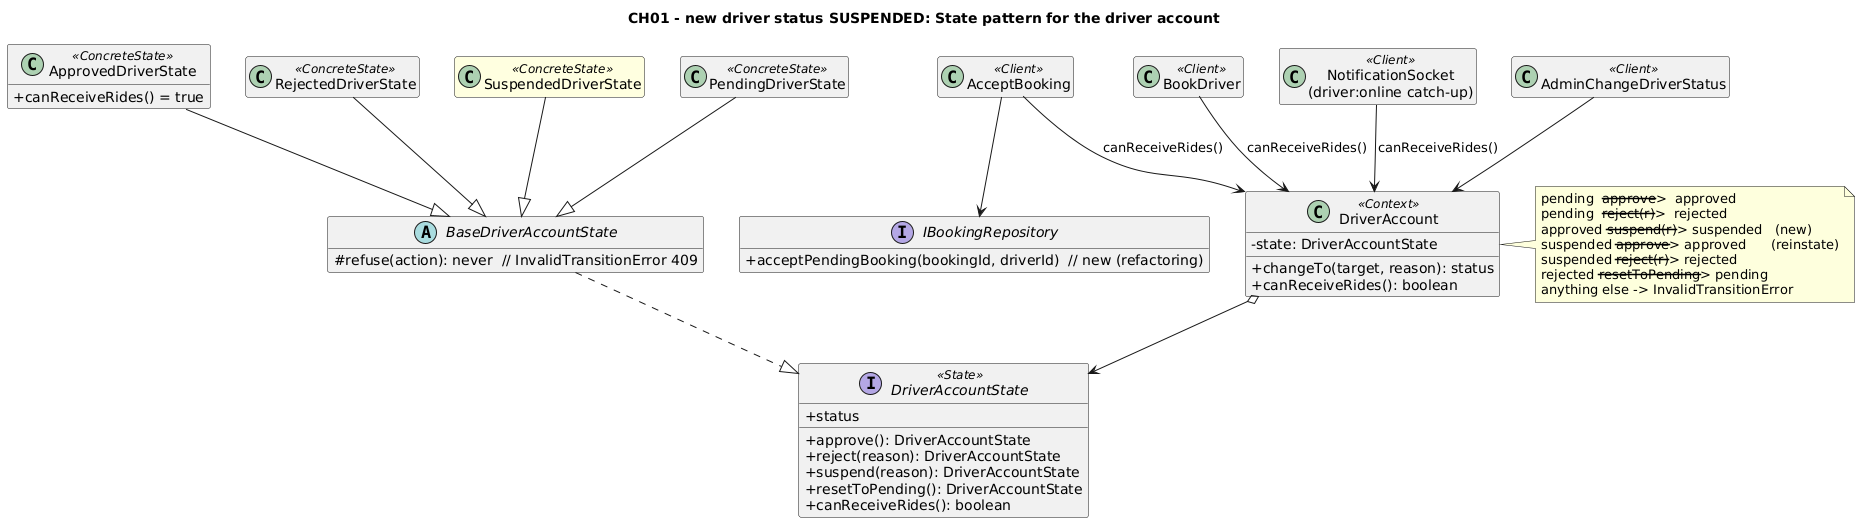
\includegraphics[width=\linewidth]{Part2/diagrams/ch01_driver_account_state.png}
\end{columns}
\end{frame}

\begin{frame}{CH02 -- ride cancellation (State + Strategy)}
\begin{columns}[T]
\column{0.4\textwidth}\small
\begin{itemize}
\item \texttt{TripLifecycle}: Pending, Confirmed, Finished -- used by cancel, status update, expiry
\item \texttt{CancellationPolicy}: rider late fee (10\%, min Rs 50 after 21:00 IST day before); driver free
\item Rider \emph{and} driver can cancel only their own rides
\item New event \texttt{booking:cancelledByDriver}
\item Tests 33/33
\end{itemize}
\column{0.6\textwidth}
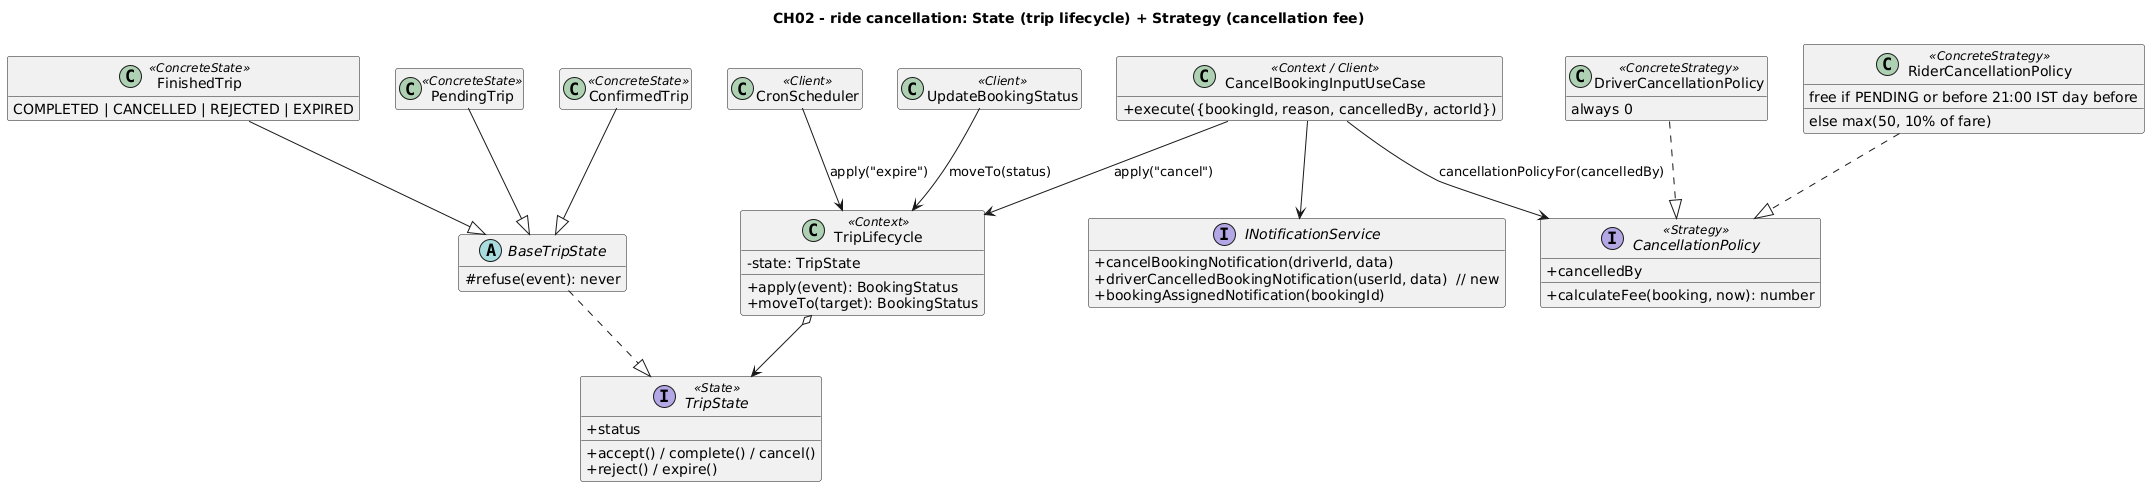
\includegraphics[width=\linewidth]{Part2/diagrams/ch02_trip_state_cancellation.png}
\end{columns}
\end{frame}

\begin{frame}{CH03 -- ride types + dynamic pricing (Strategy + Decorator)}
\begin{columns}[T]
\column{0.38\textwidth}\small
\begin{itemize}
\item New HOURLY and OUTSTATION fares; one class per ride type
\item \texttt{PeakHourSurcharge} $\times$1.25, \texttt{LowSupplySurcharge} $\times$1.2 wrap any strategy
\item \texttt{FareCalculatorService} CC 6 $\rightarrow$ 2
\item 6 baseline fare tests pass unchanged
\item Tests 41/41
\end{itemize}
\column{0.62\textwidth}
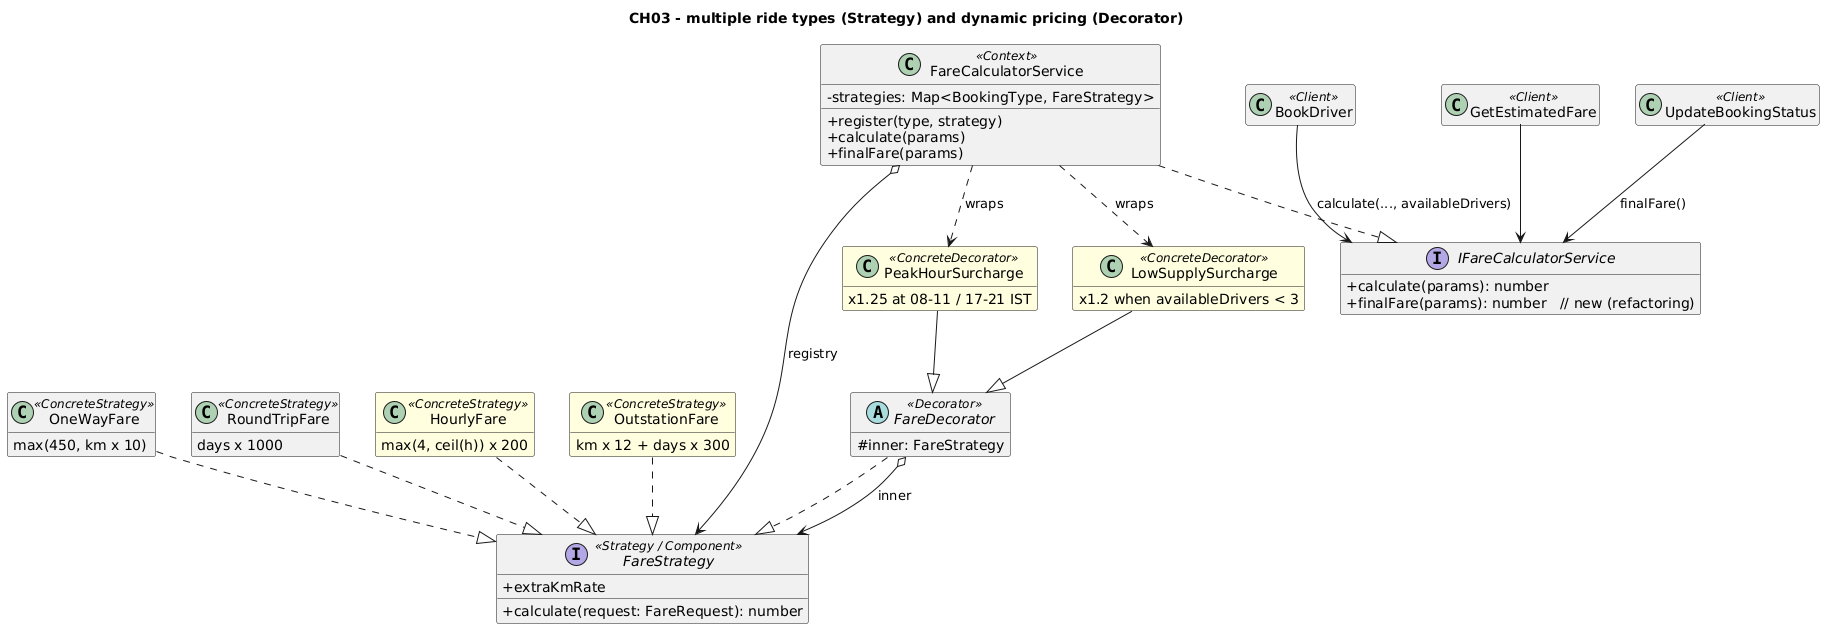
\includegraphics[width=\linewidth]{Part2/diagrams/ch03_fare_strategy_decorator.png}
\end{columns}
\end{frame}

\begin{frame}{How the pattern set changed}
\centering
\begin{tabular}{@{}lrrl@{}}\toprule Snapshot & Types & Instances & Change\\\midrule
Original & 10 & 16 & --\\
After CH01 & 11 & 17 & + State (driver account)\\
After CH02 & 12 & 19 & + State (trip), + Strategy (cancellation fee)\\
After CH03 & 12 & 21 & + Strategy (ride fare), + Decorator (dynamic pricing)\\\bottomrule
\end{tabular}

\medskip\small
Extended: notification Adapter + Observer, middleware chain, trip repository, DI. Nothing removed.\\
Cost: +448 NLOC overall; some use cases more complex (ownership, supply rules). LOC alone is not the verdict -- the defects are now tested.
\end{frame}

\begin{frame}{Part 3 -- same problem in four languages}
\small\centering
\begin{tabular}{@{}lrrrr@{}}\toprule & Java 25 & Python 3.13 & Node 22 & C++20 (g++ 13)\\\midrule
Strategy LOC / CC / ms & 57 / 3 / 103 & 51 / 3 / 60 & 47 / 3 / 49 & 69 / 3 / 2.1\\
State LOC / CC / ms & 58 / 6 / 98 & 52 / 2 / 31 & 41 / 2 / 45 & 57 / 6 / 1.9\\
Observer LOC / CC / ms & 33 / 3 / 111 & 31 / 3 / 64 & 24 / 2 / 46 & 40 / 3 / 2.3\\\bottomrule
\end{tabular}

\medskip
All 12 pass: Strategy 8/8, State 8/8, Observer 6/6. Time = median of 5 full test processes (start-up dominated).
\end{frame}

\begin{frame}{Part 3 -- what differed}
\begin{itemize}
\item \textbf{Roles:} nominal interfaces checked by the compiler (Java, C++) vs.\ \texttt{Protocol}/duck typing (Python, JS)
\item \textbf{Dispatch:} \texttt{getattr}/\texttt{state[event]()} removes the event switch (CC 2 vs 6)
\item \textbf{Ownership:} only C++ must say who owns strategies/states (\texttt{unique\_ptr}) and that the hub must not keep observers alive (\texttt{weak\_ptr})
\item \textbf{Start-up:} JVM $\approx$100\,ms, Node $\approx$47\,ms, CPython 31--64\,ms (imports matter), native $\approx$2\,ms
\end{itemize}
\end{frame}

\begin{frame}{LLM use and limitations}
\begin{itemize}
\item 10 real LLM runs (1 Claude Code, 9 ChatGPT free tier): prompt, input, raw output, verification (\texttt{prompts/}, \texttt{data/llm.csv})
\item 3 correct, 7 partial; all 12 ChatGPT-generated programs passed the fixtures, but its explanations had slips
\item ChatGPT disputed our Observer / \texttt{catchAsync} Decorator / module Singleton and found 2 open gaps (non-atomic cancel, \texttt{activePayment})
\item Every pattern accepted only from traced code + tests, never from a name or an LLM claim
\item Limitations: no live run against MongoDB/Redis/Stripe/Google; dependency drift (7 pre-existing \texttt{tsc} errors); no upstream license
\end{itemize}
\end{frame}

\end{document}
